\documentclass[a4paper,12pt]{article}


\usepackage{setspace}
\usepackage{xcolor}
\usepackage{graphicx}
\usepackage{geometry}
\usepackage{float}
\usepackage{titlesec}
\usepackage{subfigure}
\usepackage{caption}
\captionsetup{figurewithin=section}
\usepackage{amsmath}


\begin{document}

\title{\textbf{Homework 2}}
\author{Yunian Pan}
\maketitle{}

\section{Problem 1: Perceptron}
Using GD, set the max iteration to be 1000, the the evolution of binary classification error and the perceptron error with iterations from random initialization until convergence on a successful run are shown as \ref{1-1}:

\begin{figure}[h]
\centering
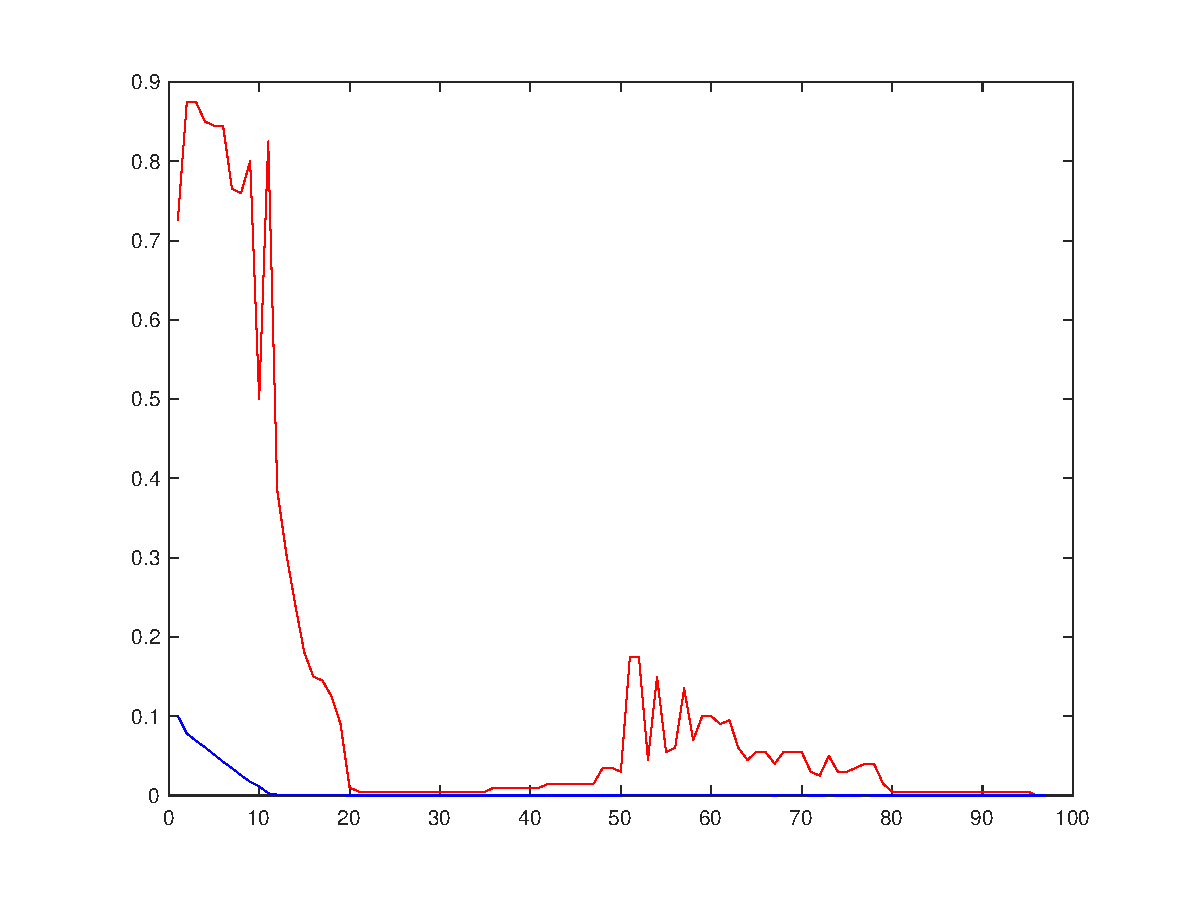
\includegraphics[width = .8\textwidth]{figure/1_1.eps}
\caption{evolution of errors with iteration}
\label{1-1}
\end{figure}

In which the red represents the classification error given by $R(\theta ) = \dfrac{1}{N} \sum_{i=1}^{N} step(-y_i \theta ^\mathsf{T} x_i)$ and the blue represents the perceptron error given by $R^{per}(\theta) = -\dfrac{1}{N} \sum_{i \in misclassified} y_i (\theta^\mathsf{T} x_i)$. And the 2D linear boundary is shown in \ref{1-2}

\begin{figure}[h]
\centering
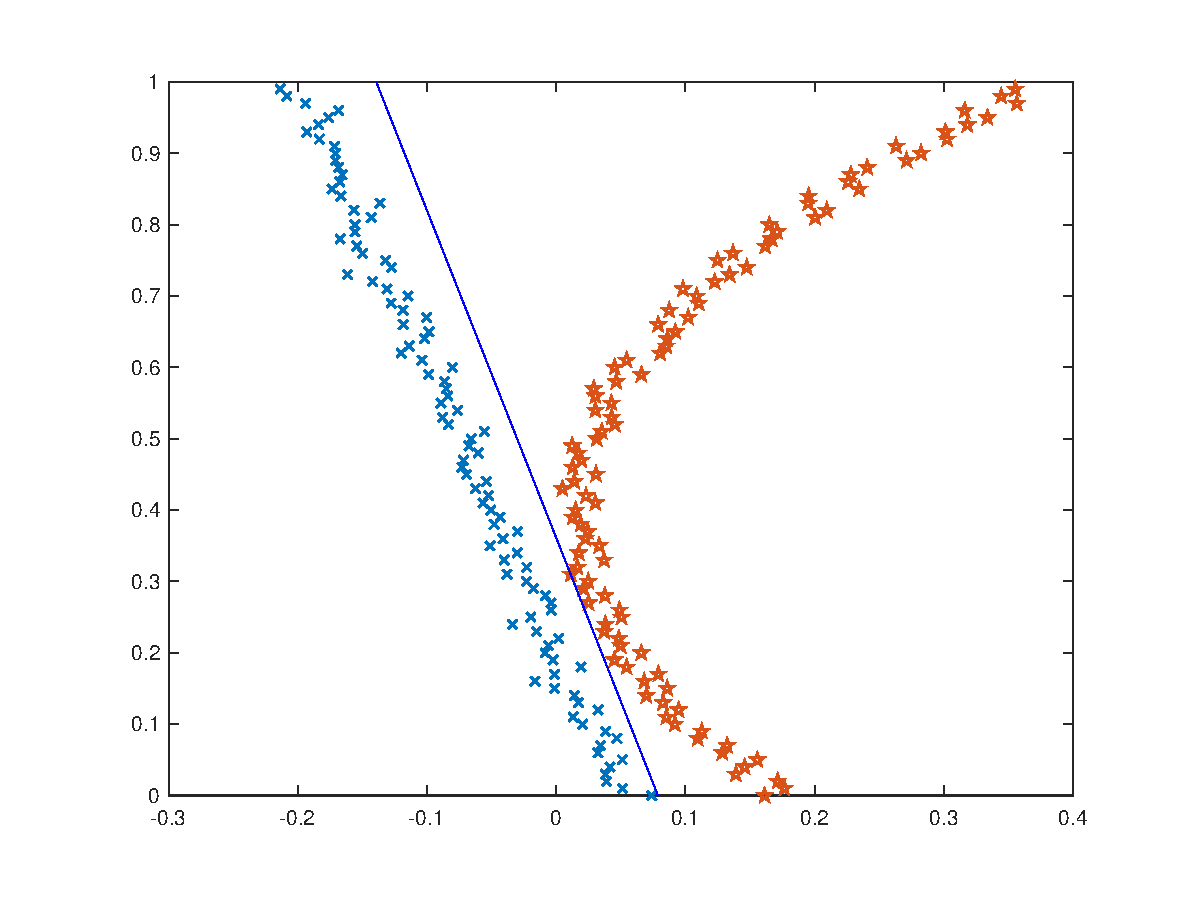
\includegraphics[width = .8\textwidth]{figure/1_2.eps}
\caption{boundary}
\label{1-2}
\end{figure}

Using SGD, the figures are shown in \ref{1-3} and \ref{1-4}, the error oscillates with time.

\begin{figure}[h]
\centering
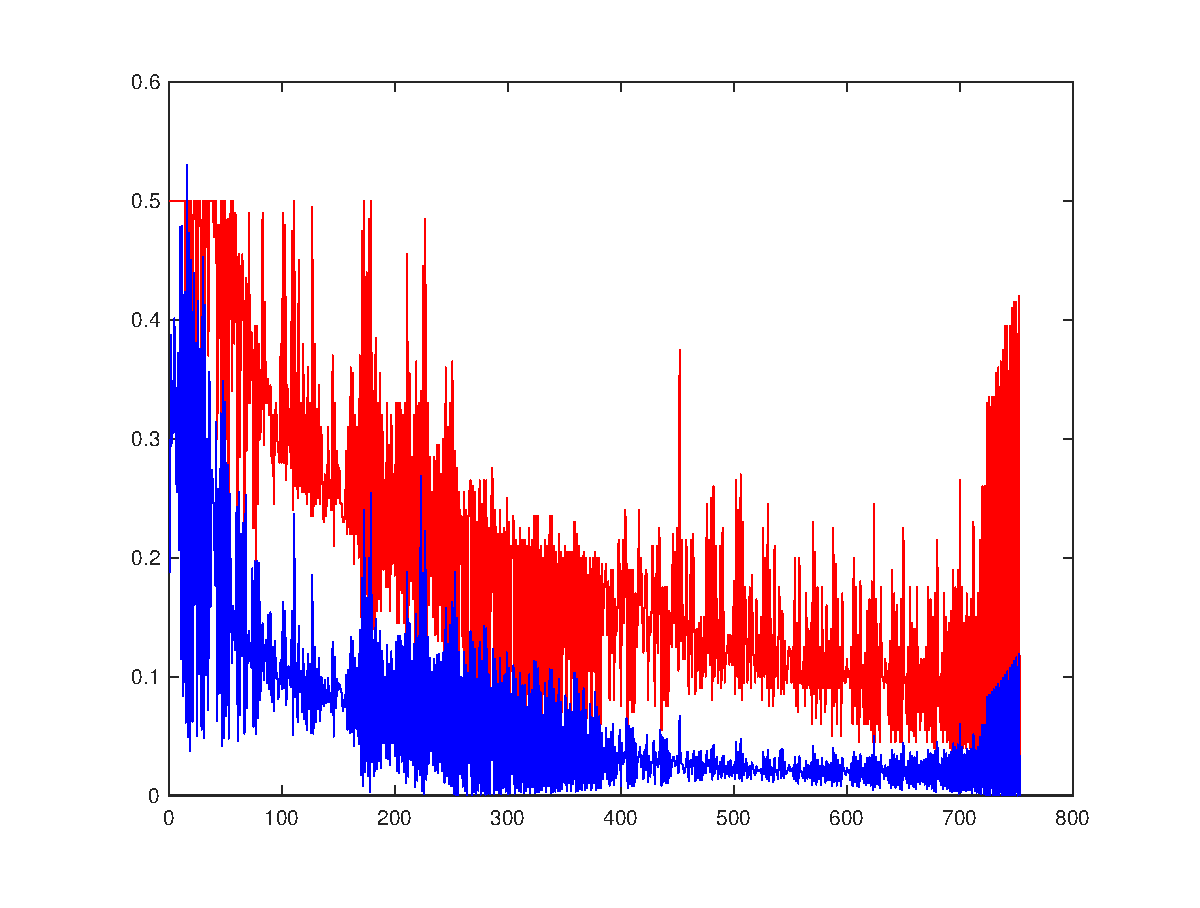
\includegraphics[width = .8\textwidth]{figure/1_3.eps}
\caption{evolution of errors with time}
\label{1-3}
\end{figure}

\begin{figure}[h]
\centering
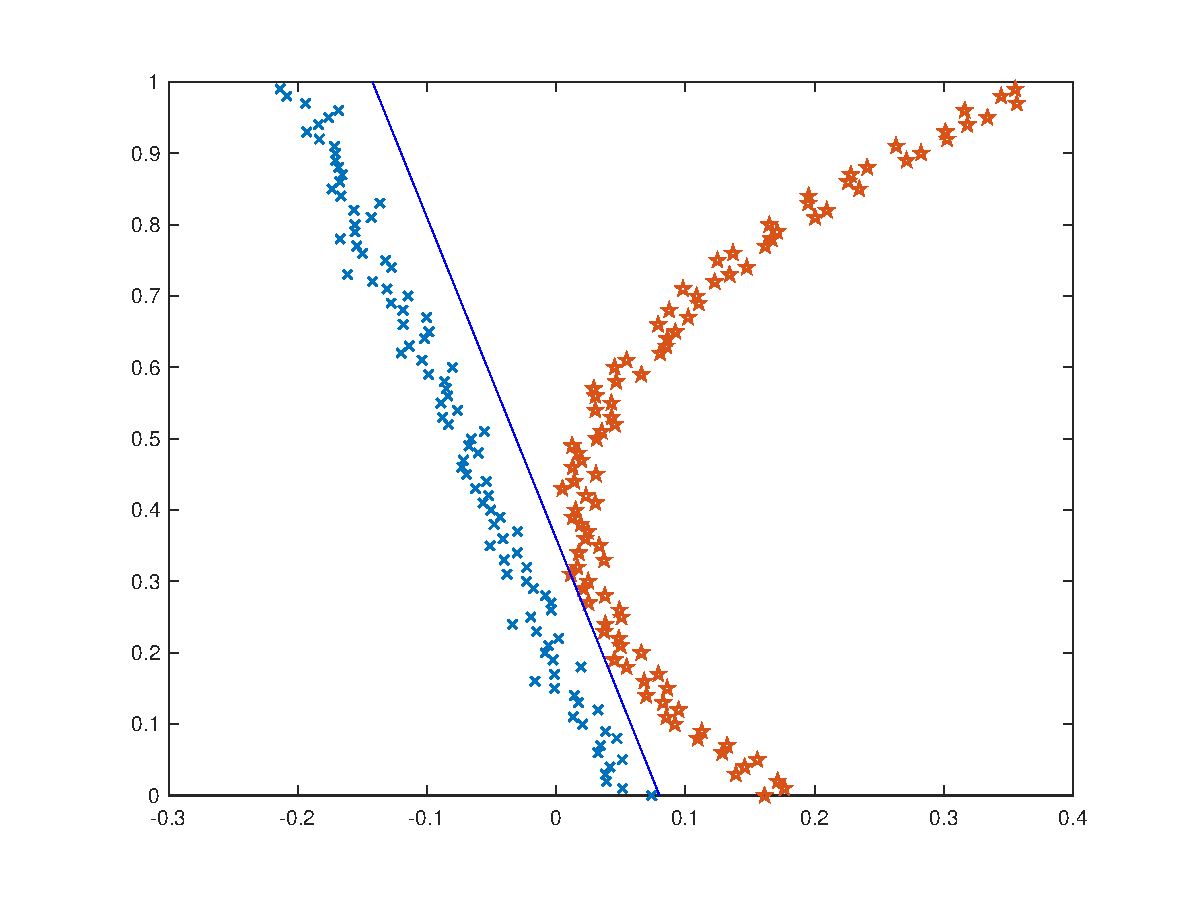
\includegraphics[width = .8\textwidth]{figure/1_4.eps}
\caption{boundary}
\label{1-4}
\end{figure}

Discussion: when the learning rate $\eta$ varies, the iteration that algorithm runs also changes, when $\eta = 1$, the max iteration varies from 60 to 140, when $\eta = 0.1$, the max iteration varies from 100 to 200, when $\eta = 0.01$, the max iteration varies from 400 to 1000 or even more, and when $\eta$ increases to 10 or 100, the max iteration falls down within 100. 

\section{Problem 2: Neural network}

\subsection{a)}

The three units can be converted to one, through simplification, $C W^{\mathsf{T}} A$ can be represented by $C [(w_2 w_6 + w_1 w_5) x_1 + (w_4 w_6 + w_3 w_5 )x_2]$ that's the same as converting the network to one unit with weights vector $\left[ w_2 w_6 + w_1 w_5, w_4 w_6 + w_3 w_5\right]^{\mathsf{T}}$, computing the same function without using any hidden units. 

\subsection{b)}

It is possible. Since it's linear operation that is represented by every layer, take the a) for example, the process is no more than

\begin{align}
\begin{bmatrix}{x_1 \quad x_2}\end{bmatrix} \begin{bmatrix}{w_2  & w_3 \\ w_4 & w_6} \end{bmatrix}  \begin{bmatrix}{w_6 \\ w_5}\end{bmatrix} = \begin{bmatrix}{x_1 \quad x_2}\end{bmatrix} \begin{bmatrix}{w_2 w_6 + w_1 w_5 \\ w_4 w_6 + w_3 w_5}\end{bmatrix} \nonumber
\end{align}

We can compute the matrix multiplication regardless of how many layers there are, and the final results can be represented by one unit.

\subsection{c)}

The final form is 
\begin{align}
Y = t\{ w_5\left[1 + \exp(w_1 X_1 + w_3 X_2)\right]^{-1} + w_6\left[1 + \exp(w_2 X_1 + w_4 X_2)\right]^{-1} \}.  \nonumber
\end{align}
It handles $X_1$ XOR $X_2$ when $W^{\mathsf{T}}$ satisfies 
\begin{align}
&w_5+w_6 < 0 \\
&w_5 / (1+ \exp(w_1 + w_3)) + w_6 / (1+ \exp(w_2+ w_4)) < 0 \\
&w_5 / (1+ \exp(w_1 )) + w_6 / (1+ \exp(w_2))> 0 \\
&w_5 / (1+ \exp(w_3 )) + w_6 / (1+ \exp(w_4))> 0 
\end{align}
Let $w_5 = 1 $, $w_6 = -2$, $w_3 = w_1$ and $w_4 = w_2$, we can easily find a couple of values that satisfy the inequality above, e.g. $w_1 = w_3 = 4$, $w_2 = w_4 = 8$.

\section{Problem 3: Backpropagation}

\subsection{case 1}

Sol: 

Given $x_i = g(y_j) = \dfrac{1}{1+e^{-\sum_j {w_{ji}y_j}}}$, and $\sum_{i}\dfrac{\partial E}{\partial x_i} = -\sum_i {(\dfrac{t_i}{x_i} - \dfrac{1 - t_i}{1 - x_i})}$ apply the chain rule, first take $x_i$ and $y_j$ as fixed to compute the gradient for $w_{ji}$, then take $z_k$ and $y_j$ as fixed to compute the gradient for $w_{kj}$ we have 
\begin{align}
\frac{\partial E}{\partial w_{ji}} & = \frac{\partial E}{\partial x_i}\frac{\partial x_i}{\partial w_{ji}}\nonumber \\
&= (\frac{1-t_i}{1- x_i} - \frac{t_i}{x_i})\frac{\partial g(w_{ji}, y_j) }{\partial w_{ji}} \nonumber \\
& = (\frac{1-t_i}{1- x_i} - \frac{t_i}{x_i}) x^2_i y_{j} e^{-\sum_j{w_{ji}y_j}} \nonumber \\
& = (\frac{1-t_i}{1- x_i} - \frac{t_i}{x_i}) x_i y_{j} (1-x_i) \nonumber \\
& = (x_i - t_i) y_j \nonumber \\
\qquad \nonumber 
\end{align}

\begin{align}
\frac{\partial E}{\partial w_{kj}} & =  \sum_{i} (\frac{\partial E}{\partial x_i}  \dfrac{\partial x_i}{\partial y_j} )\frac{\partial y_j}{\partial w_{kj}} \nonumber \\
& =  \sum_{i} \frac{\partial E}{\partial x_i}(-w_{ji}) x_i (1 - x_i) (-z_k) y_j(1- y_j)\nonumber  \\
& = \sum_{i} \frac{x_i - x_i t_i - t_i + x_i t_i}{ (1-x_i)x_i } (-(-w_{ji}) x_i (1 - x_i))(- (-z_k) y_j(1- y_j)) \nonumber \\
& = \sum_{i} (x_i - t_i) w_{ji} y_j(1- y_j) z_k \nonumber 
\end{align}

Thus, we have\qquad $\sum_{i} \dfrac{\partial E}{\partial w_{ji}} = \sum_i \delta_j^i y_j$, \qquad $\sum_{j} \dfrac{\partial E}{\partial w_{kj}} = \sum_j \delta_k^j z_k$. 

\subsection{case 2}

Sol:

Given the cross-entropy $E = -\sum_i t_i \log(x_i)$ and softmax activation function $x_i = \dfrac{e^{\sum_{j} w_{ji} y_j}}{\sum_{i} e^{\sum_{j} w_{ji}y_j}} = f(w_{11}, \ldots , w_{j1}, \ldots, w_{ji}, \ldots,  w_{jm}, \ldots , y_j, \ldots)$, we have
\begin{align}
\frac{\partial E}{\partial x_i} &= - \frac{t_i}{x_i} \nonumber \\
\quad  \nonumber \\
\frac{\partial x_m}{\partial w_{ji}} & =  \frac{y_j(\delta(i-m) e^{\sum_{j}w_{jm}y_j}( \sum_{i}e^{\sum_{j}w_{ji}y_j} ) - e^{\sum_{j}w_{jm}y_j} e^{\sum_{j}w_{ji}y_j})}{(\sum_{i} e^{\sum_{j} w_{ji}y_j})^2}   \nonumber  \\
& = y_j x_m( \delta(i-m) - x_i)  \nonumber \\
\nonumber \\
\frac{\partial E}{\partial w_{ji}} & = \sum_{m} \frac{\partial E}{\partial x_m} \frac{\partial x_m}{\partial w_{ji}}   \nonumber \\
& = \sum_{m} y_j (-\frac{t_m}{x_m}) x_m( \delta(i - m) - x_i)  \nonumber \\
& = y_j (\sum_{m} t_m \cdot x_i - t_i) \nonumber 
\end{align}
\begin{align}
\frac{\partial E}{\partial w_{kj}} & = \sum_{i}( \sum_{m} (\frac{\partial E}{\partial x_m} \frac{\partial x_m}{\partial y_j}) \frac{\partial y_j}{\partial w_{kj}} ) \nonumber \\
& = \sum_{i} (w_{ji} (\sum_{m} t_m x_i - t_i)) y_j (1 - y_j) z_k \nonumber \\
& =  \sum_{i}(\sum_{m} t_m x_i - t_i)(w_{ji} y_j(1- y_j)) z_k \nonumber
\end{align}
Here\quad$\delta_j^i = \sum_{m} t_m \cdot x_i - t_i$,\quad$\delta_k^j =  \sum_{i}(\sum_{m} t_m x_i - t_i)(w_{ji} y_j(1- y_j))$. For both cases, \quad$w^{t+1} = w^{t} - \eta \dfrac{\partial E}{\partial w^{t}}$.

\section{Problem 4: VC dimension}

Sol:

The VC dimension is 7. we can draw a circumcircle in the 2D plane and arrange the points on the circle, for a set of 7 points labeled by $\{+1, -1\}$, the max cardinality of convex hull is $\left[\dfrac{7}{2}\right] = 3$, let the 3 points be the vertexes, which indicates that we can always find a triangle that contains the 3 points and has no intersection with other points; For a set of 8 points, the max convex hull becomes 4 points, take the labeling \{+1, -1, +1, -1, +1, -1, +1, -1\} which is the most complex condition for example, there is no triangle that can shatter them, because there will be one point either outside or inside the convex hull that can't be determined, as illustrated in \ref{VC}.

\begin{figure}
\centering
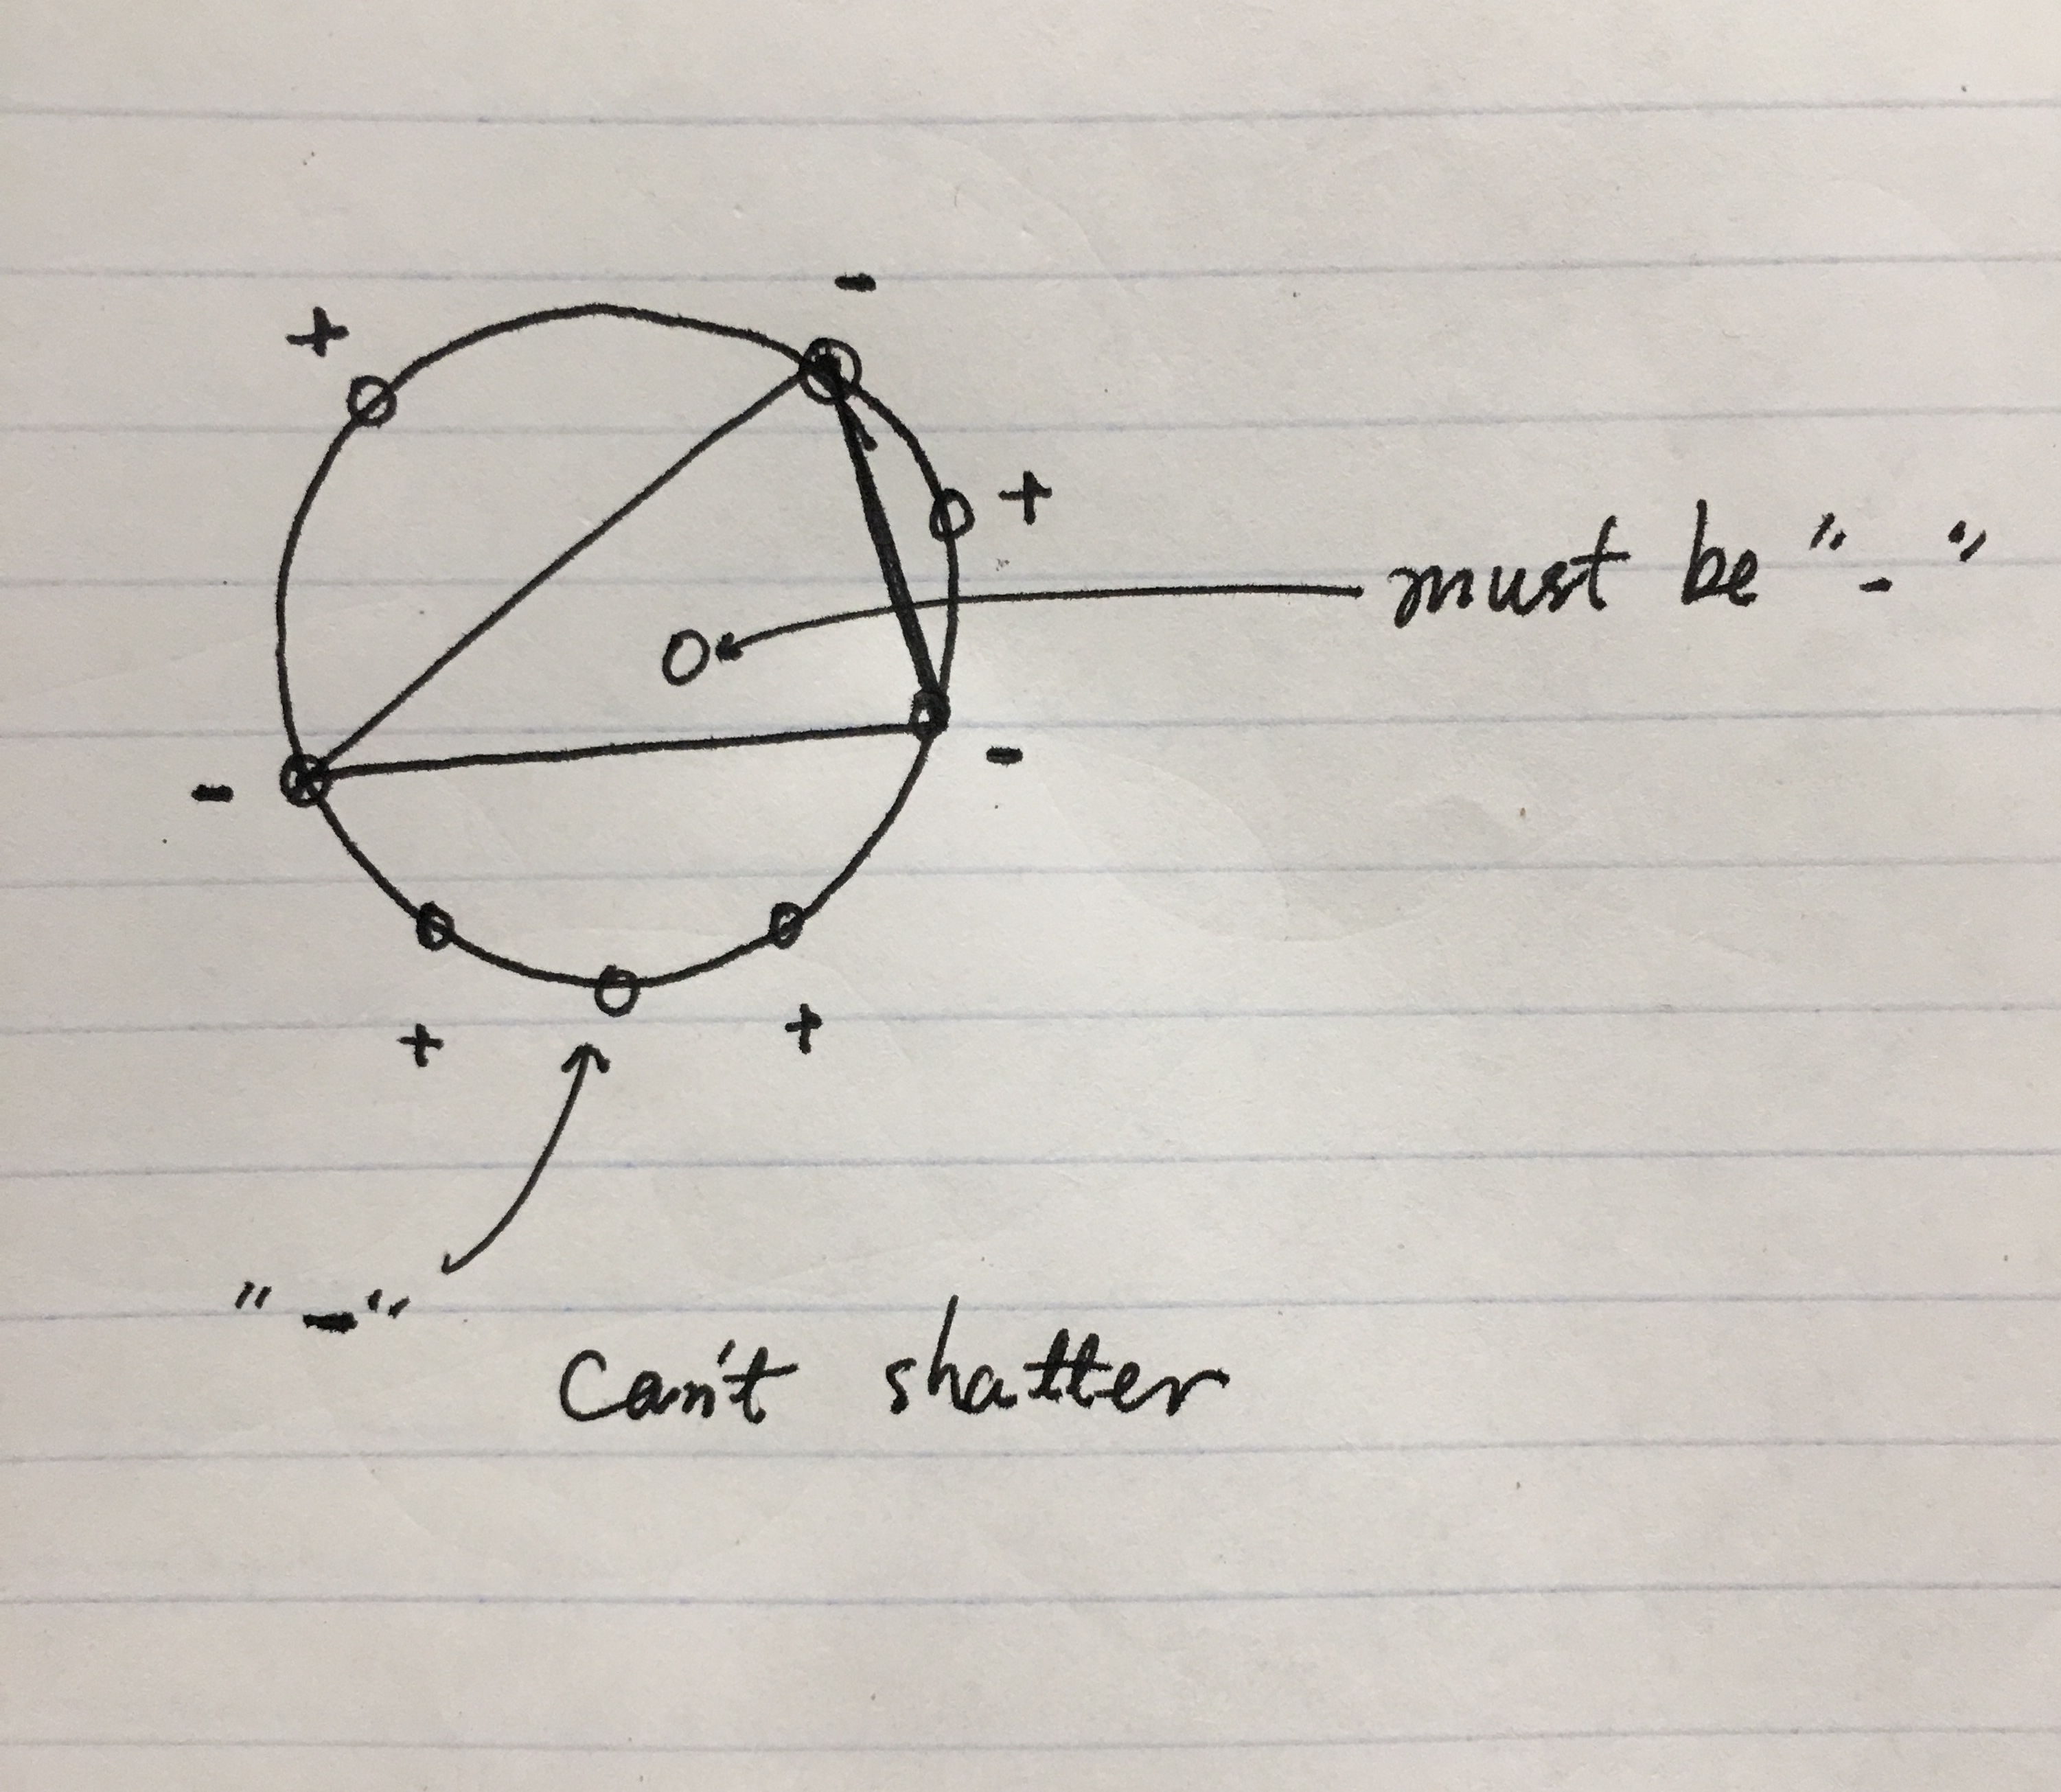
\includegraphics[width = .5\textwidth]{figure/VC.jpeg}
\caption{illustration}
\label{VC}
\end{figure}

Therefore, $VC(H) = 7$.

\end{document}